% Denne fil er inkluderet i udtraekning_af_regioner.tex
{

Floodfill finder i sin enkelthed områder i et billede, som har en farve
der ligger inde for en vis afvigelse af den originale farve. Der vælges
en pixel i billedet som har en farve angivet ved en RGB-værdi. Ud fra
denne pixel findes de fire tilstødende pixels i lodret og vandret bane,
som vist i figur \ref{floodfill1}.

\begin{figure}[!h]
    \begin{center}
        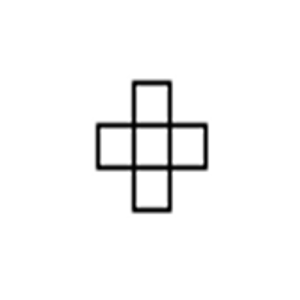
\includegraphics[scale=0.42,angle=0]{afsnit/vores_implementation/billeder/flood_fill/floodfill1}
    \end{center}
    \caption[]{Måden floodfill arbejder med pixels i billedet}
    \label{floodfill1}
\end{figure}

\subsubsection{Metode}
De følgende 3 skridt beskriver hvordan floodfillmetoden virker i et
billede.

\begin{enumerate}
    \item Algoritmen starter med at markere den midterste pixel (vores
        startpixel) med et rødt flag, som angiver at denne pixel bliver
        farvet. Nabopixels får et blåt flag, som angiver at de skal
        kontrolleres for om deres farve er indenfor afvigelsen. Blå flag
        sættes kun hvis en pixel ikke har noget flag i forvejen. Se
        figur \ref{floodfill2}.
    \item Hver pixel med et blåt flag kontrolleres for om deres
        farve ligger indenfor afvigelsen. Hvis farven er indenfor
        afvigelsen, bliver denne pixel sat i en liste og markeret med et
        grønt flag og et tal. Se figur \ref{floodfill3}
    \item En pixel med grønt flag tages ud af listen og bliver sat til
        den nye startpixel. Skridt $1$ og $2$ bliver gentaget til der
        ikke er flere grønne flag. Se figur \ref{floodfill4}
\end{enumerate}

\begin{figure}[!h]
    \begin{center}
        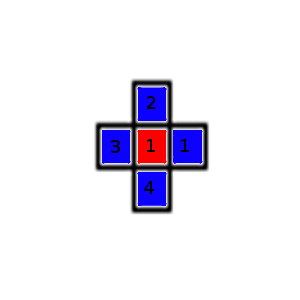
\includegraphics[scale=0.42,angle=0]{afsnit/vores_implementation/billeder/flood_fill/floodfill2}
    \end{center}
    \caption[]{Pixels efter første skridt i algoritmen. Den røde pixel
    er vores startpixel. Pixels markeret med blåt skal kontrolleres for
    deres farve. Numrene angiver rækkefølgen de bliver gennemgået.}
    \label{floodfill2}
\end{figure}

\begin{figure}[!h]
    \begin{center}
        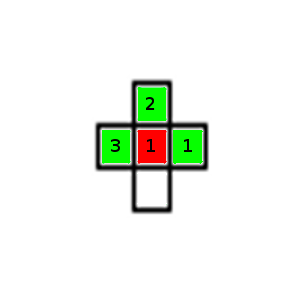
\includegraphics[scale=0.42,angle=0]{afsnit/vores_implementation/billeder/flood_fill/floodfill3}
    \end{center}
    \caption[]{Pixels efter andet skridt i algoritmen. De pixels som har
    en farve der ligger indenfor afvigelsen bliver markeret med et grønt
    flag og tildelt et tal som angiver rækkefølgen. I denne illustration
    er den nederste pixel ikke blevet farvet grøn. Den var før blå, men
    da den ikke ligger indenfor afvigelsen mister den sit flag.}
    \label{floodfill3}
\end{figure}

\begin{figure}[!h]
    \begin{center}
        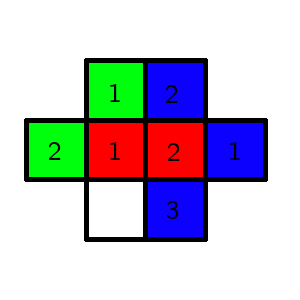
\includegraphics[scale=0.42,angle=0]{afsnit/vores_implementation/billeder/flood_fill/floodfill4}
    \end{center}
    \caption[]{Pixels efter skridt 3 og et nyt skridt 1. Vi har valgt
    den grønne pixel med det laveste tal fra figur \ref{floodfill3} som
    ny startpixel. Nye pixels markeret med blåt mangler at blive
    kontrolleret.}
    \label{floodfill4}
\end{figure}

På denne måde itererer metoden sig igennem alle de pixels som ligger
inde for en vis afgivelse fra startfarven. Denne metode kan gøres på to
måder; Enten kan man regne afvigelsen ud fra farven som vores startpixel
har eller man kan regne den fra den nye pixel som bliver fundet i tredje
skridt. Det skal bemærkes at den pixel, som i figur \ref{floodfill3}
mister sit blå flag, godt kan blive taget i betragtning igen senere når
vi vælger en ny startpixel. En pixel kan dog højst blive taget i
betragtning i alt fire gange fordi den har fire tilstødende pixels.

\subsubsection{Eksempler}
Vi vil nu vise nogle eksempler på hvordan denne metode virker i praksis.
Vi vil i dette afsnit manipulere billedet vist i figur \ref{bathers}.
Dette billede er valgt, da det har været brugt i flere argumenter for at
det gyldne snit er at finde i
malerkunsten\cite{GoldenNumber}\cite{RatioArt}.  Endvidere er maleriet
interessant at teste på, da det er udført i det der kaldes pointilistisk
stil, hvilket vil sige at maleriet faktisk består af en masse små
prikker. I de fem billeder vist i figur \ref{dot_ff_fixed_7_7},
\ref{dot_ff_var_7_7}, \ref{dot_ff_fixed_10_10}, \ref{dot_ff_var_10_10}
og \ref{dot_ff_var_9_9} bruges floodfill på den pixel i midten af den
røde prik. Den tilladte afvigelse gives som en tupel $(lo, up)$ med en
værdier for henholdsvis hvor meget RGB-værdien må falde og stige. Det
anbefales at studere figurene og den tilhørende tekst.

% Det her billede opfører sig underligt mht. scale :/
\begin{figure}[!h]
    \begin{center}
        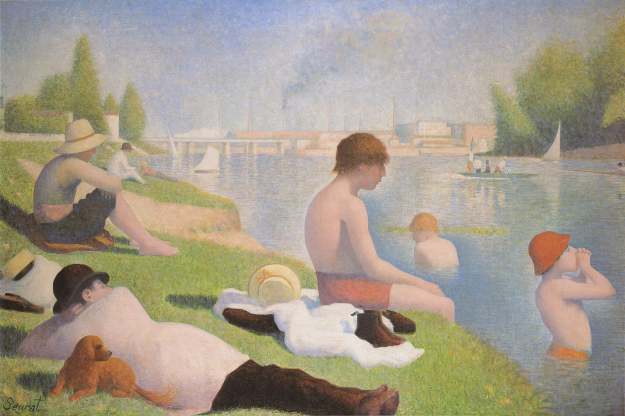
\includegraphics[scale=8]{afsnit/vores_implementation/billeder/flood_fill/seurat_bathers}
    \end{center}
    \caption[George Seurat: \emph{Bathers at Asnieres} - 1884]{George
    Seurat: \emph{Bathers at Asnieres} - 1884\\Originalt billede}
    \label{bathers}
\end{figure}

\begin{figure}[!h]
    \begin{center}
        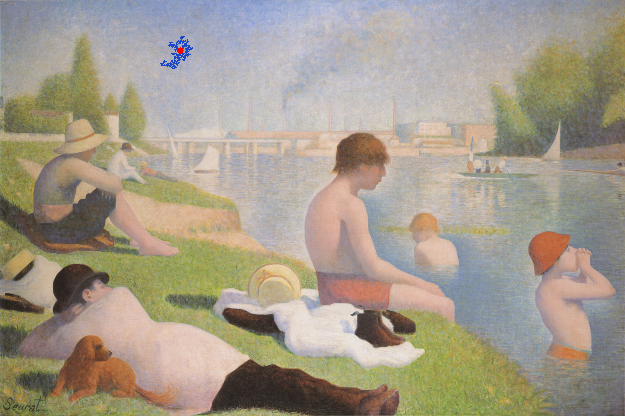
\includegraphics[scale=0.49]{afsnit/vores_implementation/billeder/flood_fill/dot_ff_fixed_7_7}
    \end{center}
    \caption[]{Floodfill hvor der kun sammenlignes med farven på den
    originale pixel med afvigelsen $(7,7)$.}
    \label{dot_ff_fixed_7_7}
\end{figure}

\begin{figure}[!h]
    \begin{center}
        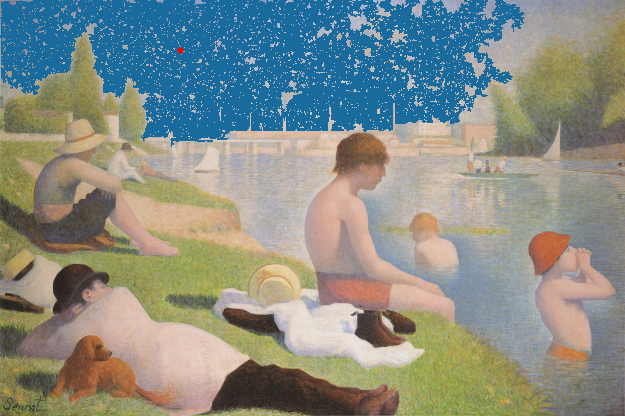
\includegraphics[scale=0.49]{afsnit/vores_implementation/billeder/flood_fill/dot_ff_var_7_7}
    \end{center}
    \caption[]{Floodfill hvor der sammenlignes med farven på den nye
    startpixel. Afvigelsen er sat til $(7,7)$ ligesom i figur
    \ref{dot_ff_fixed_7_7}. Det ses at vi nu dækker et meget større
    areal.}
    \label{dot_ff_var_7_7}
\end{figure}

\begin{figure}[!h]
    \begin{center}
        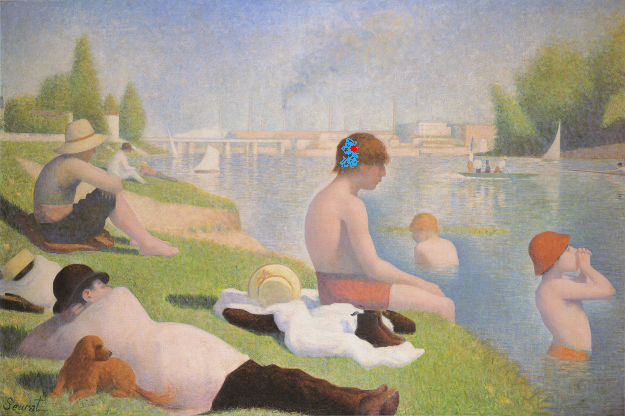
\includegraphics[scale=0.49]{afsnit/vores_implementation/billeder/flood_fill/dot_ff_fixed_10_10}
    \end{center}
    \caption[]{Floodfill med udgangspunkt i en ny pixel og kun
    sammenligning med den originale pixel. Den tilladte afvigelse er på
    $(10,10)$.}
    \label{dot_ff_fixed_10_10}
\end{figure}

\begin{figure}[!h]
    \begin{center}
        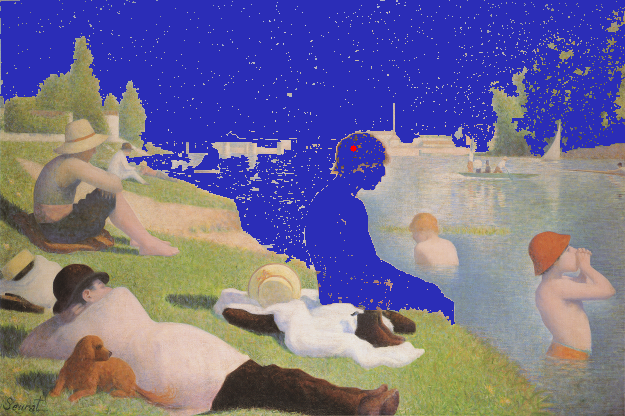
\includegraphics[scale=0.49]{afsnit/vores_implementation/billeder/flood_fill/dot_ff_var_10_10}
    \end{center}
    \caption[]{Floodfill med samme udgangspunkt og afvigelse som i figur
    \ref{dot_ff_fixed_10_10}, men der sammenlignes nu med den nye
    startpixel. Med en større tilladt afvigelse, breder floodfill sig
    meget mere og smelter både himmel, hav og dreng sammen.}
    \label{dot_ff_var_10_10}
\end{figure}

\begin{figure}[!h]
    \begin{center}
        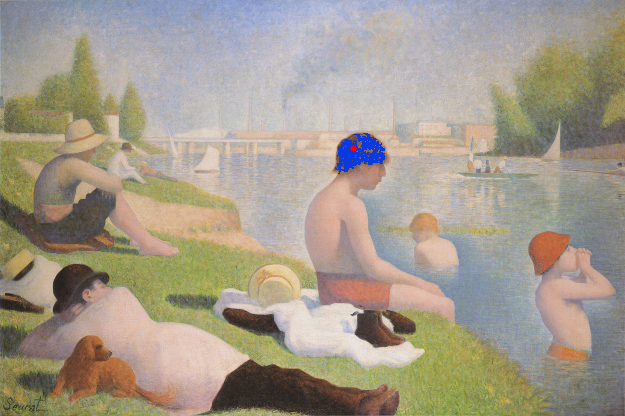
\includegraphics[scale=0.49]{afsnit/vores_implementation/billeder/flood_fill/dot_ff_var_9_9}
    \end{center}
    \caption[]{Floodfill med samme udgangspunkt som i figur
    \ref{dot_ff_fixed_10_10} og \ref{dot_ff_var_10_10}. Her bruges igen
    sammenligning med ny startpixel, men nu med en afvigelse på $9,9$.
    Denne lille ændring er nok til, at vi holder os pænt indenfor den
    region som udgøres af drengens hår.}
    \label{dot_ff_var_9_9}
\end{figure}

\subsubsection{Hvilken metode passer bedst?}
Som nævnt ovenfor og illustreret i billederne er der to måder vi kan
bruge floodfill på. Hvis man vælger at regne varianten ud fra den første
startpixel, ses det at metoden vil indskrænke sig meget og ikke komme
ind i alle hjørner af en region. Til gengæld har denne fremgangsmåde
sværere ved at krydse kanter og på den måde komme ind i en ny region.

Vælger man at ændre varianten efter den nye startpixel, ses det at man
vil male større regioner. Da denne fremgangsmåde hele tiden tilpasser
varianten, kan man medtage regioner der langsomt skifter farve. Et godt
eksempel ses i figur \ref{dot_ff_var_10_10}, hvor drengens krop og
bukser bliver set som sammenhængende. Dette er interessant især med
hensyn til digitale billeder af malerier, da solen eller blitzens
refleksion kan påvirke billedets farver. Af samme grund er den
fremgangsmåde heller ikke særlig følsom overfor kanter, hvilket
resulterer i at man let kommer til at gå ind i andre regioner.

Vi har valgt at benytte os af den sidstnævnte metode, da den efter vores
mening giver det bedste resultat. Vi vurderer, at det at tage højde for sol og
små farveskift, vægter højere end at være sikker på at vi ikke går ud
over kanterne. Vi vil senere beskrive hvordan vi på anden vis sikrer at
vi beholder kanterne.

Som illustreret i billederne skal vi dog stadig tage højde for hvordan
vi vil sætte tærskelværdierne. Indtil videre bliver de sat efter hvad
der giver det bedste resultat grafisk.

%For at få denne metode til at virke på 25000 billeder, hvor en del af
%billederne ikke har samme farvetone eller er blevet falmet, må der
%for hvert billede udregnes hvad for en varians i farve der skal bruges.

}

% vim: set tw=72 spell spelllang=da:
